\begin{center}
	{\Large \textbf{Formas de Electrización}}
\end{center}
%%objetivos
\section{Objetivos}
\begin{itemize}
	\item Comprobar experimentalmente las formas de electrización.
	\item Estudiar la relación entre electrones y protones.
	\item Desarrollar habilidades en el manejo de datos experimentales. 
\end{itemize}

%%intruduccuión
\section{Introducción}
Un cuerpo está cargado eléctricamente cuando este posee un exceso o deficiencia de electrones, sin embargo ¿Cómo es que un cuerpo llega a cargarse eléctricamente? Todo este proceso es gracias a las diversas formas de electrización que existen, entre las más conocidas: frotamiento, contacto e inducción. Donde un cuerpo no cargado se convierte en uno cargado eléctricamente gracias a las formas ya mencionadas.

%%marco teórico
\section{Marco Teórico}
\subsection{Electrización por frotamiento}
Ocurre al momento de frotar un cuerpo neutro en las mismas condiciones; para ello cada cuerpo tiene que ser un material diferente, en este caso el laboratorio se usara un paño de tela y un pedazo de vidrio, que al momento de friccionar o frotar  uno de ellos cuerpo va empezar a ceder electrones y el cuerpo que gana los electrones quedará cargado.

\subsection{Electrización por contacto}
Según \cite{guzman2007} “La carga es transferida al electroscopio cuando la varilla cargada toca el bulbo. Entonces, cuando una varilla con carga opuesta se acerca al bulbo, las hojas se colapsan y se juntan. El electroscopio neutro se toca con una varilla cargada negativamente; las cargas son transferidas al bulbo (p.1)”\\
\begin{figure}[h]
	\centering
	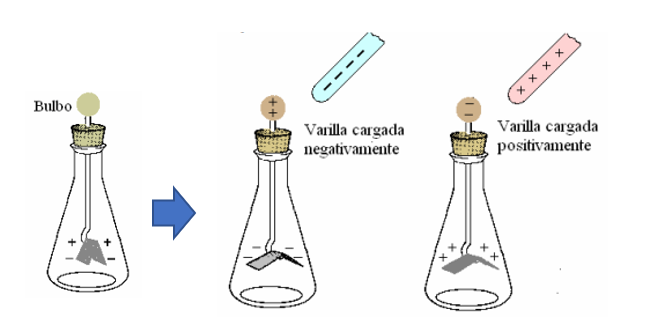
\includegraphics[width=10cm, height=8cm]{imagenes/guzman.png}
	\caption{Electrización por contacto}
\end{figure}\\
La electrización por contacto es la transferencia de electrones o protones entre dos cuerpos que uno de ellos se encuentra cargado a otro con carga neutra o en equilibrio. Este fenómeno ocurre cuando al momento de poner en contacto los dos cuerpos con las características ya mencionadas.  Y la carga se distribuye entre los cuerpos, y cuerpo que no estaba cargado empieza a ganar mayor cantidad de electrones o protones, y el cuerpo cargado pierde. Así dos cuerpos se encuentran cargados de manera negativa o positiva. Cuerpo cargado negativamente, es cuando un cuerpo se encuentra con exceso de electrones, y defecto de protones; al momento del contacto gano electrones.

\subsection{Electrización por inducción}
" La electrización por influencia o inducción es un efecto de las fuerzas eléctricas. Debido a que éstas se ejercen a distancia, un cuerpo cargado positivamente en las proximidades de otro neutro atraerá hacia sí a las cargas negativas, con lo que la región próxima queda cargada negativamente. Si el cuerpo cargado es negativo entonces el efecto de repulsión sobre los electrones atómicos convertirá esa zona en positiva. En ambos casos, la separación de cargas inducida por las fuerzas eléctricas es transitoria y desaparece cuando el agente responsable se aleja suficientemente del cuerpo neutro."  \cite{etitudela2016}
\begin{figure}[h]
	\centering
	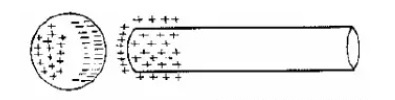
\includegraphics[width=8cm, height=4cm]{imagenes/induccion.jpg}
	\caption{Electrización por inducción}
\end{figure}\\
Es cuando un cuerpo con carga neutra es atraído por un cuerpo que está cargado ya sea positiva o negativo, puesto que el cuerpo cargado está alterado por el desbalance de carga que tiene. Al momento de atraer se produce la distribución de cargas, así el cuerpo neutro queda electrizado por la carga del cuerpo cargado.

%%materiales
\section{Materiales}
\begin{table}[h]
	\begin{center}
		\begin{tabular}{|c|c|c|}
			\hline
			Electroscopio & Pedazo de vidrio & Esfera metálica \\
			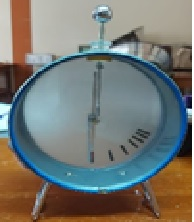
\includegraphics[width=4cm, height=3cm]{imagenes/electoscopio.jpg} & 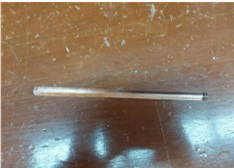
\includegraphics[width=4cm, height=3cm]{imagenes/pedazovidrio.jpg} & 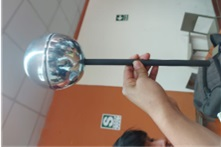
\includegraphics[width=4cm, height=3cm]{imagenes/esferametalica.jpg}\\
			\hline
			Generador Van de Graff & Pedazo de tela & Rehilete \\
			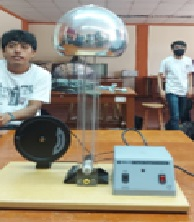
\includegraphics[width=4cm, height=3cm]{imagenes/generador.jpg} & 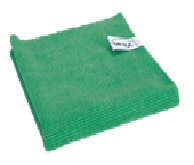
\includegraphics[width=4cm, height=3cm]{imagenes/tela.jpg} &
			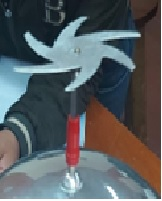
\includegraphics[width=4cm, height=3cm]{imagenes/rehilete.jpg}\\
			\hline
		\end{tabular}
	\end{center}
\end{table}

%%procedimeiento o parte experimental
\section{Procedimiento o parte experimental}
\subsection{Actividad 01: por frotamiento}
\begin{itemize}
	\item Se dispone de un pedazo de vidrio, un pedazo de tela y un electroscopio. 
	\item El pedazo de vidrio debe ser frotado con el pedazo de tela, de manera intensa.
	\item El proceso del frotamiento se muestra en la Figura 03. 
	\begin{figure}[h]
		\centering
		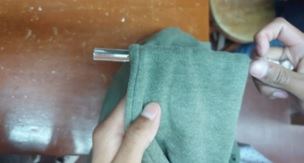
\includegraphics[width=3cm, height=4cm]{imagenes/porfrotamiento.jpg}
		\caption{Experimento por frotamiento}
	\end{figure}
	\item Posteriormente, coloque el pedazo de vidrio en la parte superior del electroscopio (esfera metálica). De forma que estos choquen. Ver Figura 04.
	\begin{figure}[h]
		\centering
		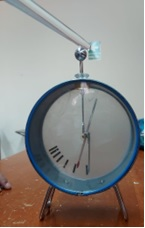
\includegraphics[width=3cm, height=4cm]{imagenes/lecturadeelctrometro.jpg}
		\caption{Lectura del electroscopio}
	\end{figure} 
	\item Como se observa en la figura 04, la lámina de oro se cambió de posición, lo cual indica que el pedazo de vidrio está cargado eléctricamente.
\end{itemize}

\subsection{Actividad 02: por Contacto}
\begin{itemize}
	\item Se dispone de una esfera metálica, un generador de Van de Graff y un electroscopio. 
	\item Antes de realizar el procesamiento debemos encargarnos de que la esfera metálica no tenga carga eléctrica.
	\item Del mismo modo hacemos uso del generador de Van de Graff, y lo empezamos a cargar eléctricamente (en este caso el generador funcionaba con un enchufe).
	\item Posteriormente ponemos en contacto la esfera metálica con el Van de Graff, tal y como se muestra en la figura 05.
	\begin{figure}[h]
		\centering
		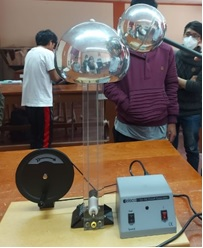
\includegraphics[width=3cm, height=4cm]{imagenes/porcontacto.jpg}
		\caption{Proceso de contacto de las esferas}
	\end{figure}\\
\end{itemize}
\begin{itemize}
	\item Al realizar dicho contacto llevamos la esfera metálica al electroscopio, donde sabremos si realmente se cargó. Ver figura 06.
	\begin{figure}[h]
		\centering
		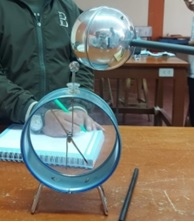
\includegraphics[width=3cm, height=4cm]{imagenes/electrometro2.jpg}
		\caption{Lectura del electroscopio}
	\end{figure}\\
\end{itemize}

\subsection{Actividad 03: por inducción}
\begin{itemize}
	\item Se dispone del generador de Van de Graff y un rehilete. 
	\item En primer lugar, colocamos el rehilete encima del Van de Graff.
	\item Posteriormente, conectamos el Van de Graff, para que este sea cargado eléctricamente y del mismo modo cargue y haga girar el rehilete. Ver figura 07.
	\begin{figure} [h]
		\centering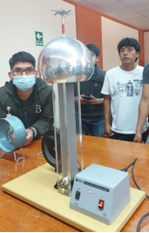
\includegraphics[width=3cm, height=4cm]{imagenes/porinduccion.jpg}
		\caption{Rehilete girando por la presencia de energía eléctrica}
	\end{figure}\\
\end{itemize}

%%análisis de resultados
\section{Análisis de resultados}
\subsection{Actividad 01: por frotamiento}
A inicios del experimento el pedazo de vidrio se encuentra en estado neutro, es decir sin carga eléctrica. Al momento de realizar el frotamiento, los electrones de la tela se liberan y dirigen hacia el pedazo de vidrio. En este caso el pedazo de tela al perder electrones, éste llega a cargarse positivamente mientras que el vidrio al recibir electrones logra cargarse negativamente.
Posteriormente, colocamos el pedazo de vidrio en la esfera metálica del electroscopio, y este al ser de metal (conductor de energía) atrae los electrones y estos se dirigen a las varillas del electroscopio donde, “la repulsión electrostática entre las cargas positivas hace que la varilla gire, separándose del soporte central” \cite{martinez}

\subsection{Actividad 02: por contacto}
En este experimento, al conectar el generador de Van de Graff genera un campo eléctrico, puesto que existe una interacción entre cargas positivas y negativas. Del otro lado tenemos una esfera metálica sin carga eléctrica. Ambos elementos al juntarlos se transfieren cargas, y al finalizar la transmisión ambos quedan con la misma carga eléctrica. Es decir, al final la carga del generador de Van debe ser igual al de la esfera metálica. 
Posteriormente la esfera metálica fue dirigida al electroscopio, donde gracias a la figura 06 se comprueba que si existe energía eléctrica.

\subsection{Actividad 03: por inducción}
Al momento de experimentar esta forma de electrización, se tuvo que tomar en cuenta que es lo que pasaba con el rehilete. Al iniciar el experimento, el rehilete no poseía ninguna carga y este al ser sometida al generador de Van de Graff se cargó y se dio el efecto puntas, “cuando la superficie presenta una punta, las cargas se concentran en dicha punta, por lo tanto se produce un campo eléctrico más intenso, se ionizan las moléculas que rodean la punta (el aire se vuelve conductor), y se produce una fuga de cargas por la punta, lo que se conoce como efecto de punta”, \cite{electrostática}, es por esta razón que el rehilete obtiene un movimiento. 

%%conclusiones y recomendaciones
\section{Conclusiones y recomendaciones}
\subsection{Conclusiones}
\begin{itemize}
	\item En conclusión, este trabajo, nos ha ayudado a afianzar, consolidar y ampliar nuestros conocimientos aprendidos acerca de las formas de electrización y como es que podemos experimentarlos en la vida real, ya que se realizó el bosquejo exacto de estas formas de electrificar a un cuerpo.
	\item Al concluir con los tres (3) experimentos se llegó a comprender que un cuerpo es cargado eléctricamente, gracias a la existencia de los protones y electrones y es como estos llegan a transferirse, en el primer caso electrización por frotamiento, nos dimos cuenta de que mientras más frotábamos más fuerte iba a ser la concentración de electrones y por ende mayor energía eléctrica, puesto que se señala que si un cuerpo tiene deficiencia o exceso de electrones este está cargado eléctricamente. En el segundo caso, electrización por contacto, tan solo basta que un elemento conductor eléctrico este en contacto con otro no cargado, para que este al momento de juntarse obtengan la misma carga, distribuidas equitativamente. En tercer caso, electrización por inducción, el conductor que vendría a ser el que cede la carga eléctrica al cuerpo no cargado, sin embargo, a diferencia del segundo caso ambas masas terminan con cargas distintas, es decir, uno queda positivamente y el otro negativamente.
	\item Asimismo, se adquirió una mayor destreza y cuidado en el manejo de los diversos instrumentos.
\end{itemize}

\subsection{Recomendaciones}
\begin{itemize}
	\item Se debe comprobar el buen estado de los instrumentos a utilizar, para que así podamos tener una mejor proyección del experimento que estamos realizando.
	\item Los materiales se debe tratar con cuida para no sufrir algún inconveniente o algún accidente al momento de experimentar.
	\item Seguir las reglas del laboratorio y usar los implementos necesarios para no poder sufrir alguna descarga eléctrica durante la realización del experimento.
\end{itemize}

